\documentclass[a4paper,12pt]{article}
\usepackage[utf8]{inputenc}
\usepackage[ngerman]{babel}
\usepackage[a4paper, left=2.5cm, right=2.5cm]{geometry}
\usepackage{graphicx}
\usepackage{subcaption}
\usepackage{fancyhdr}
\usepackage{pdfpages}
\pagestyle{fancy}
\usepackage{multirow}
\usepackage{amsmath}
\lhead{Messtechnik Labor}
\chead{}
\rhead{Gruppe 2}

\begin{document}
	%Titelseite
	
\includepdf{tp1.pdf}
	
	\noindent
	\textbf{\Large Rechtliches} \\ \\
	Ich bestätige hiermit, dass alle hier verwendeten Messergebnisse und Interpretationen von uns selbst erstellt wurden. Es wurden keine anderen Quellen als die hier schriftlich angegeben verwendet.
	\setcounter{page}{2}
	
	\newpage
	%Inhaltsverzeichnis
	\tableofcontents
	
	\newpage
	\section{Einleitung}
	In dieser Laborübung wurden folgende Themengebiete behandelt:
	\begin{itemize}
		\item Spannungs-,Strom- und Widerstandsmessung
		\item Spannungsmessung mit dem Oszilloskop
		\item Messwerke 
	\end{itemize}
	Der erste Teil der Übung bestand darin den Innenwiderstand eines Voltmeters und eines Amperemeter, sowie deren Einfluss auf die jeweilige Messung. Anschließend sollte bei beiden Messungen auch eine Messbereichserweiterung realisiert werden. Die letzte Aufgabe des ersten Teiles bestand darin einen niederohmigen und hochohmigen Widerstand mit unterschiedlichen Arten zu bestimmen. \\
	Die Aufgabe im zweiten Teil der Übung bestand darin, das Verhalten eines Tastkopfes zu untersuchen. Anschließend wurden Messungen von unterschiedliche Wechselspannungssignalen und zur Bestimmung der Spitze- und RMS-Werte durchgeführt. \\
	Am Ende der Laborübung untersuchten wir zwei unterschiedliche Messwerke und machten uns mit deren Funktionsprinzip, Eigenschaften und Anwendungsgebieten vertraut.

	\newpage
	\section{Übungsdurchführung}
	\subsection{Spannungs-,Strom- und Widerstandsmessung}
	\subsubsection{Spannungsmessung}
	\underline{\textbf{Aufgabenstellung}} \\ \newline
	\noindent
	In dieser Aufgabe soll eine Messung für die Bestimmung des Innenwiderstand eines Voltmeters, dessen Einfluss auf die Spannungsmessung und eine Messbereichserweiterung durch einen Spannungsteiler durchgeführt werden. \\ \\
	\noindent
	\underline{\textbf{Bestimmung des Innenwiderstandes}} \\ \\
	Um den Innenwiderstand des Voltmeters zu bestimmen, wurde die Schaltung wie in \\
	Abbildung 1 zu sehen auf einem Steckbrett aufgebaut und mit \(10V\) versorgt.
	\begin{figure}[h]
		\centering
		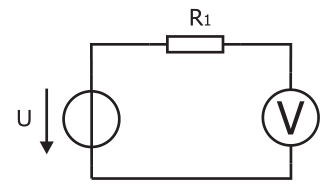
\includegraphics[width=8cm]{img/Voltmeter_Innenwiderstand}
		\caption{Schaltung zur Messung des Innenwiderstands des Voltmeters}
	\end{figure}
	\newline
	Um Ungenauigkeiten bei der Berechnung des Innenwiderstandes zu vermeiden wurde der Widerstand \(R_1\) mit einem Ohmmeter bestimmt. Dieser hatte einen Wert von \(100.7k\Omega\). Laut Netzgerät betrug die Versorgungsspannung \(10.01V\). Der Innenwiederstand kann nun mithilfe eines Spannungsteilers bestimmt werden, welcher lautet:
	\[
		R_V = \frac{U_V}{U_{R1}}R_1
	\]
	\newpage
	\begin{table}[h]
		\centering
		\begin{tabular}{|c|c|c|c|c|c|}
			\hline
			\multirow{2}{*}{$U[V]$} & \multirow{2}{*}{$R_1[k\Omega]$} & \multirow{2}{*}{$U_V[V]$} & \multirow{2}{*}{$U_{R1}[V]$} & \multirow{2}{*}{$I[\mu A]$} & \multirow{2}{*}{$R_i[M\Omega]$} \\
			&  &  &  &  &  \\ \hline
			\multirow{2}{*}{$10.01$} & \multirow{2}{*}{$100.7$} & \multirow{2}{*}{$0.90$} & \multirow{2}{*}{$0.10$} & \multirow{2}{*}{$1.09$} & \multirow{2}{*}{$9.045$} \\
			&  &  &  &  &  \\ \hline
		\end{tabular}
		\caption{Auswertung von 2.1.1 Punkt 1}
	\end{table}
	\noindent
	Es wurde ein Innenwiderstand des Voltmeters erwartet, damit dieser geringe Einflüsse auf die Messung mit sich trägt. Das zu untersuchenden Voltmeter hat einen Innenwiderstand von ca $9M\Omega$, was unsere Erwartung bestätigt. Ein ideales Voltmeter besitzt einen unendlich großen Widerstand, damit das Messgerät überhaupt keinen Einfluss auf die Messung hat. Dieser Innenwiderstand ist jedoch nicht realisierbar. \\
	
	\noindent
	\underline{\textbf{Einfluss des Voltmeters auf die Spannungsmessung}} \\ \newline
	\noindent
	Um den Einfluss des Voltmeters auf die Messung zu untersuchen, wird die Schaltung aus Abbildung 1 um ein 2 Voltmeter erweitert. Dies ist in Abbildung 2 zu sehen. Zuerst wird die Spannung am ersten Voltmeter abgelesen. Im nächsten Schritt wird ein zweites Voltmeter parallel an das erste dazugeschaltet und beide Werte abgelesen.
	\begin{figure}[h]
		\centering
		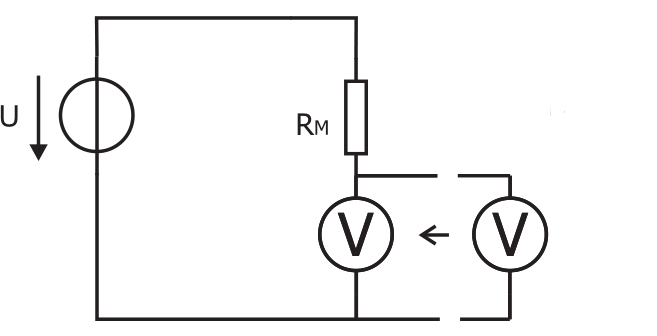
\includegraphics[width=10cm]{img/Einfluss_Voltmeter}
		\caption{Schaltung zur Messung des Einflusses eines Voltmeters auf die Spannungsmessung}
	\end{figure}
	\newline
	Nimmt man an, dass die beiden Voltmeter einen identischen Innenwiderstand besitzen, lässt sich der Spannungsabfall wie folgt berechnen:
	\[
		U_V = U \frac{\frac{R_i}{2}}{R_M + \frac{R_i}{2}}
	\]
	\begin{table}[h]
		\centering
		\begin{tabular}{|c|c|c|}
			\hline
			\multirow{2}{*}{$U[V]$} & \multirow{2}{*}{$U_{V1}[V]$} & \multirow{2}{*}{$U_{V2}[V]$} \\
			&  &  \\ \hline
			\multirow{2}{*}{$10.01$} & \multirow{2}{*}{$9.8$} & \multirow{2}{*}{$9.81$} \\
			&  &  \\ \hline
		\end{tabular}
		\caption{Auswertung von 2.1.1 Punkt 2}
	\end{table}
	\newpage
	\noindent
	\underline{\textbf{Messbereichserweiterung durch einen Spannungsteiler}}\\
	\newline
	\noindent
	Um den Messbereich der Spannungsmessung zu erweitern, können die Effekte des Spannungsteilers genutzt werden. Der Schaltungsaufbau ist aus Abbildung 3 zu entnehmen.
	%Schalungsaufbau einfügen
	\begin{figure}[h]
		\centering
		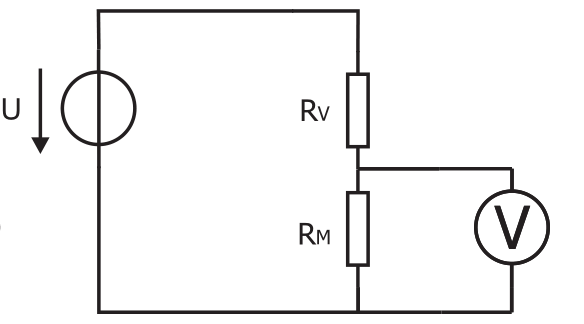
\includegraphics[width=10cm]{img/Messbereich_Voltmeter}
		\caption{Schaltung zur Messbereichserweiterung für ein Voltmeter}
	\end{figure}
	\newline
	Bei dieser Messaufgabe wurden zwei gleich große Widerstände gefordert.
	Jedoch standen nicht gleich große Widerstände im Labor zur Verfügung. Der Faktor $f_{ME}$ zur Messbereichserweiterung wird wie folgt berechnet:
	\[
		f_{ME} = \frac{U}{U_{RM}} = \frac{R_M}{R_M + R_V}
	\]
	\newline
	Um den genauen Faktor zu bestimmen wurde der Widerstand $R_V$ genauso wie der Widerstand $R_M$ mit dem Ohmmeter gemessen.
	\begin{table}[h]
		\centering
		\begin{tabular}{|c|c|c|c|c|}
			\hline
			\multirow{2}{*}{$U[V]$} & \multirow{2}{*}{$U_{RM}[V]$} & \multirow{2}{*}{$R_M[k\Omega]$} & \multirow{2}{*}{$R_V{k\Omega}$} & \multirow{2}{*}{$f_{ME}[1]$} \\
			&  &  &  &  \\ \hline
			\multirow{2}{*}{$10.01$} & \multirow{2}{*}{$5.033$} & \multirow{2}{*}{$100.7$} & \multirow{2}{*}{$102.8$} & \multirow{2}{*}{$1.988$} \\
			&  &  &  &  \\ \hline
		\end{tabular}
		\caption{Auswertung von 2.1.1 Punkt 3}
	\end{table}
	\newpage
	\subsubsection{Strommessung}
	\underline{\textbf{Aufgabenstellung}}\\ \\
	In diesem Teil der Übung, soll der Innenwiderstand eines Amperemeters und dessen Einfluss auf die Strommessung gemessen. Zum Schluss soll w eine Messbereichserweiterung mithilfe eines Stromteilers realisiert werden. \\ \\
	\noindent
	\underline{\textbf{Bestimmung des Innenwiderstandes}} \\ \\
	Zur Bestimmung des Innenwiderstand eines Amperemeters wird die Schalung aus Abbildung 1 einfach um ein Amperemeter erweitert (Abbildung 4).
	\begin{figure}[h]
		\centering
		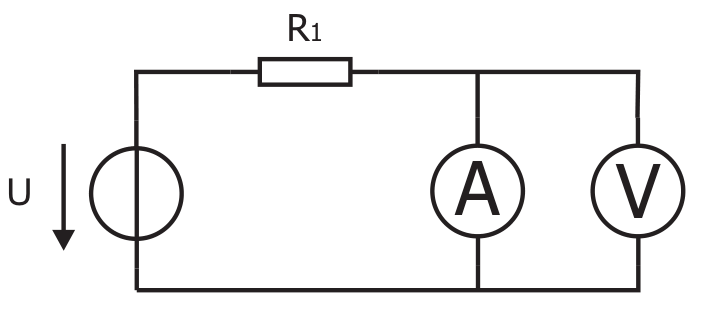
\includegraphics[width=10cm]{img/Amperemeter_Innenwiderstand}
		\caption{Schaltung zur Messung des Innenwiderstandes eines Amperemeters}
	\end{figure}
	\newline
	Um wieder Ungenauigkeiten bei der Berechnung des Innenwiderstandes zu vermeiden, wurde der Widerstand $R_1$ mit einem Ohmmeter gemessen. Gefordert war ein Widerstand mit dem Wert $4.7k\Omega$. Der gemessene Wert betrug $4,709k\Omega$. Um die Messung durchzuführen wird die Spannung bei der Spannungsversorgung solange erhöht, bis am Amperemeter ein Wert von $500 \mu A$ angezeigt wird. Anschließend kann mit den abgelesenen Werten von Ampere- und Voltmeter der Innenwiderstand des Amperemeters berechnet werden. \\
	\[
		R_i = \frac{U_V}{I_A}
	\]
	\newpage
	\begin{table}[h]
		\centering
		\begin{tabular}{|c|c|c|}
			\hline
			\multirow{2}{*}{$U_A[V]$} & \multirow{2}{*}{$I[\mu A]$} & \multirow{2}{*}{$R_i[k\Omega]$} \\
			&  &  \\ \hline
			\multirow{2}{*}{$1.624$} & \multirow{2}{*}{$500.2$} & \multirow{2}{*}{$3.246$} \\
			&  &  \\ \hline
		\end{tabular}
	\caption{Auswertung von 2.1.2 Punkt 1}
	\end{table}
	\noindent
	Grundsätzlich wurde ein sehr kleiner Innenwiderstand bei einem Amperemeter erwartet. Die Messung hat jedoch ergeben, dass dieser im $k\Omega$ befindet. Der Wert des Innenwiderstand in diesen Wertebereich lässt sich damit begründen, dass beim Amperemeter ein Messbereich für $\mu A$ eingestellt wurde, welcher den Innenwiderstand des Messgerätes erhöht, sodass bei geringen Strömen ein relativ kleiner Spannungsabfall am Amperemeter auftritt. \\ \\
	\underline{\textbf{Einfluss des Amperemeters auf die Strommessung}} \\ \\
	\noindent
	Der Messaufbau ist Abbildung 5 zu entnehmen.
	\begin{figure}[h]
		\centering
		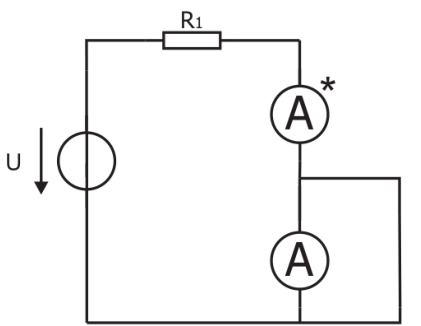
\includegraphics[width=8cm]{img/Einfluss_Amperemeter}
		\caption{Schaltung zur Messung des Einflusses eines Amperemeters auf die Strommessung}
	\end{figure}
	\newline
	Anfangs soll das zweite Amperemeter mit einem Bügel kurzgeschlossen werden. Nun führt führt man dieselbe Messung wie im vorherigen Punkt durch. Anschließend wird der Bügel entfernt und es werden die Werte der beiden Amperemeter aufgenommen. Der Faktor $f_A$ soll nun ermittelt werden.
	Bei der Messung  mit dem Kurzschlussbügel muss bei der Spannungsquelle eine Spannung von $3.98V$ eingestellt werden, damit man am ersten Amperemeter ein Strom von $500\mu A$ angezeigt wird.
	\newpage
	\begin{table}[h]
		\centering
		\begin{tabular}{|c|c|c|c|c|}
			\hline
			\multirow{2}{*}{$I_1[\mu A]$} & \multirow{2}{*}{$R_{ges1}[k\Omega]$} & \multirow{2}{*}{$I_2[\mu A]$} & \multirow{2}{*}{$R_{ges2}[k\Omega]$} & \multirow{2}{*}{$f_A[1]$} \\
			&  &  &  &  \\ \hline
			\multirow{2}{*}{$500.4$} & \multirow{2}{*}{$7.953$} & \multirow{2}{*}{$362.3$} & \multirow{2}{*}{$10.985$} & \multirow{2}{*}{$0.658$} \\
			&  &  &  &  \\ \hline
		\end{tabular}
		\caption{Auswertung von 2.1.2 Punkt 2}
	\end{table}
	\noindent
	Verwendete Formel:
	\[
		f_A = \frac{R_{ges1}}{R_{ges2}} = \frac{I_2}{I_1}
	\]
	\newline
	\underline{\textbf{Messbereichserweiterung durch einen Stromteiler}}\\ \\
	Nun soll ein Stromteiler realisiert werden um eine Messbereichserweiterung zu realisieren. Hierfür wurde zum zweiten Amperemeter ein Widerstand , der $10k\Omega$ haben sollte, parallel geschaltet. Der ausgemessene Widerstand betrug $9.87k\Omega$. Der exakte Messaufbau ist Abbildung 6 zu entnehmen.
	\begin{figure}[h]
		\centering
		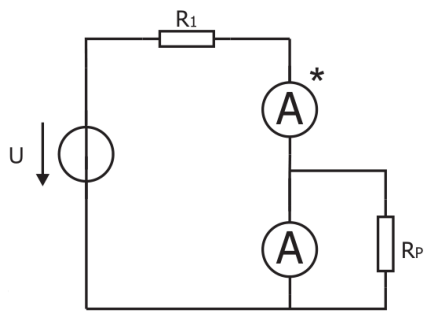
\includegraphics[width=8cm]{img/Messbereich_Amperemeter}
		\caption{Schaltung zur Messbereichserweiterung für ein Amperemeter}
	\end{figure}
	\newline
	Nun wird bei der Spannungsquelle die Spannung wieder solange erhöht, bis am ersten Amperemeter (in Abb.6 mit * zu sehen) wieder $500\mu A$ angezeigt werden. Es soll nun der Faktor $f_{ME}$ dieser Messbereichserweiterung ermittelt werden.
	\[
		f_{ME} = \frac{I_1}{I_2} = \frac{R_p}{R_p + R_i}
	\]
	\newpage
	\begin{table}[h]
		\centering
		\begin{tabular}{|c|c|c|c|}
			\hline
			\multirow{2}{*}{$R_p[k\Omega]$} & \multirow{2}{*}{$I*[\mu A]$} & \multirow{2}{*}{$I[\mu A]$} & \multirow{2}{*}{$f_{ME}[1]$} \\
			&  &  &  \\ \hline
			\multirow{2}{*}{$9.87$} & \multirow{2}{*}{$500.4$} & \multirow{2}{*}{$382.2$} & \multirow{2}{*}{$0.7657$} \\
			&  &  &  \\ \hline
		\end{tabular}
		\caption{Auswertung von 2.1.2 Punkt 3}
	\end{table}
	\subsubsection{Widerstandsmessung}
	\underline{\textbf{Aufgabenstellung}} \\ \\
	Hier bestand die Aufgabe darin, den genauen Wert eines nieder- und hochohmigen Widerstand mittels verschiedener Messmethoden zu bestimmen. \\ \\
	\underline{\textbf{Strom- und spannungsrichtig Messen}} \\ \\
	Der ohmsche Widerstand wird hier mit dem Ohmschen Gesetz bestimmt, indem man die gemessene Spannung durch den gemessenen Strom dividiert. Wie vorher festgestellt, verfälschen die Messgeräte das Messergebnis, deswegen gibt es die Möglichkeit die Messung strom- oder spannungsrichtig durchzuführen. Die Messaufbauten sind in den Abbildungen 7 und 8 zu sehen.
	\begin{figure}[h]
		\centering
		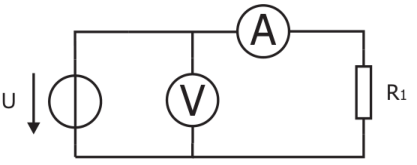
\includegraphics[width=8cm]{img/Stromrichtig}
		\caption{Schaltung zur stromrichtigen Widerstandsmessung}
	\end{figure}
	\begin{figure}[h]
		\centering
		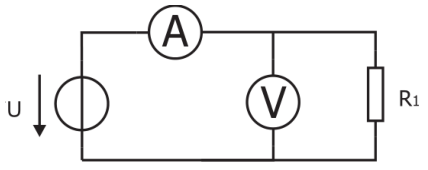
\includegraphics[width=8cm]{img/Spannungsrichtig}
		\caption{Schaltung zur spannungsrichtigen Widerstandsmessung}
	\end{figure}
	\newpage
	\noindent
	Es wird erwartet die für kleine Widerstände, die spannungsrichtige Messung vorteilhaft wäre, da der Strom der über das Voltmeter fließt, relativ klein gegenüber dem Strom der direkt über dem Widerstand fließt. Dagegen ist die stromrichtige Messung vorteilhaft bei großen Widerständen, da die anliegende Spannung am Amperemeter gegenüber der anliegenden Spannung am Widerstand vernachlässigbar klein ist. Diese zwei Messverfahren wurden mit beiden Widerständen durchgeführt.
	\begin{table}[h]
		\centering
		\begin{tabular}{|c|c|c|c|c|c|c|}
			\hline
			\multirow{2}{*}{} & \multirow{2}{*}{$U[V]$} & \multirow{2}{*}{$I[mA]$} & \multirow{2}{*}{$R_{berechnet}[\Omega]$} & \multirow{2}{*}{$U[V]$} & \multirow{2}{*}{$I[mA]$} & \multirow{2}{*}{$R_{berechnet}[\Omega]$} \\
			&  &  &  &  &  &  \\ \hline
			\multirow{2}{*}{nomineller Wert} & \multirow{2}{*}{$-$} & \multirow{2}{*}{$-$} & \multirow{2}{*}{$100\Omega$} & \multirow{2}{*}{$-$} & \multirow{2}{*}{$-$} & \multirow{2}{*}{$100k\Omega$} \\
			&  &  &  &  &  &  \\ \hline
			\multirow{2}{*}{spannungsrichtige M.} & \multirow{2}{*}{$4.987$} & \multirow{2}{*}{$49$} & \multirow{2}{*}{$101.77$} & \multirow{2}{*}{$4.853$} & \multirow{2}{*}{$47.53\mu$} & \multirow{2}{*}{$102.103k$} \\
			&  &  &  &  &  &  \\ \hline
			\multirow{2}{*}{stromrichtige M.} & \multirow{2}{*}{$4.994$} & \multirow{2}{*}{$49$} & \multirow{2}{*}{$101.91$} & \multirow{2}{*}{$4.997$} & \multirow{2}{*}{$47.11\mu$} & \multirow{2}{*}{$106.070k$} \\
			&  &  &  &  &  &  \\ \hline
			\multirow{2}{*}{Multimetermesssung} & \multirow{2}{*}{$-$} & \multirow{2}{*}{$-$} & \multirow{2}{*}{$99.7$} & \multirow{2}{*}{$-$} & \multirow{2}{*}{$-$} & \multirow{2}{*}{$100.7k$} \\
			&  &  &  &  &  &  \\ \hline
		\end{tabular}
		\caption{Auswertung von 2.1.3}
	\end{table}
	\newline
	Bei dem $100k\Omega$ Widerstand stimmen sowohl spannungs- als auch stromrichtig ziemlich  gut überein. Die folgt vermutlich daraus, der der zu messende Widerstand noch klein gegenüber dem Innenwiderstand des Voltmeters ist. Bei dem $100\Omega$ ist zwischen beiden Messverfahren kaum ein Unterschied zu erkennen, was nicht unseren Erwartungen entspricht. Dies könnte daran liegen, dass das Amperemeter nicht im $\mu A$-Bereich eingestellt war und deswegen der Innenwiderstand des Amperemeters klein genug war, um die Messung kaum zu verfälschen.
	\newpage
	\subsection{Spannungsmessung mit dem Oszilloskop}
	\subsubsection{Tastkopf}
	\underline{\textbf{Aufgabenstellung}}\\ \\
	Hier soll das Verhalten eines Tastkopfes untersucht. Genau im Fall das er unter-, überkompensiert oder abgeglichen ist. \\ \\
	\underline{\textbf{Verhalten bei einem Rechtecksignal}} \\ \\
	Hier wird der Tastkopf an das Oszilloskop angeschlossen und mit der vom Oszilloskop bereitgestellten Rechteckspannung versorgt. Nun wird an der Schraube solange gedreht bis der Tastkopf einmal über-, unterkompensiert oder abgeglichen ist. Die einzelnen Spannungsverläufe werden mit den Oszilloskop aufgenommen.
	\begin{figure}[h]
		\begin{subfigure}{7cm}
			\centering
			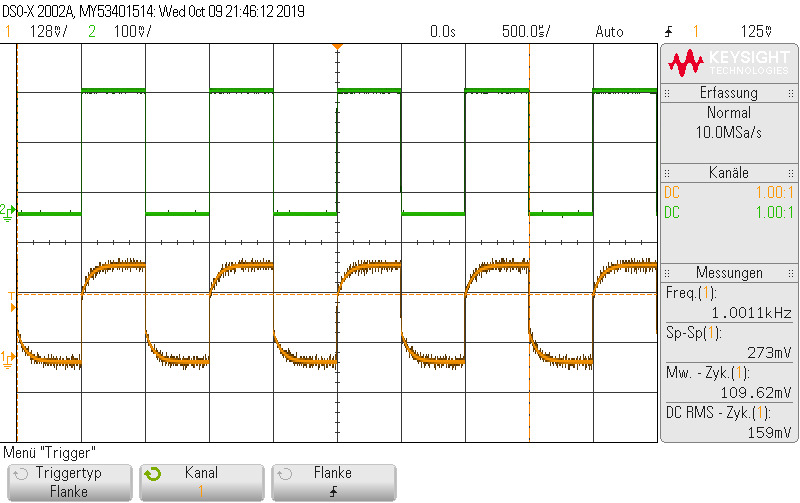
\includegraphics[width=8cm]{img/Unterkompensiert}
			\subcaption{unterkompensiert}
		\end{subfigure}
		\hspace{2.5cm}
		\begin{subfigure}{7cm}
			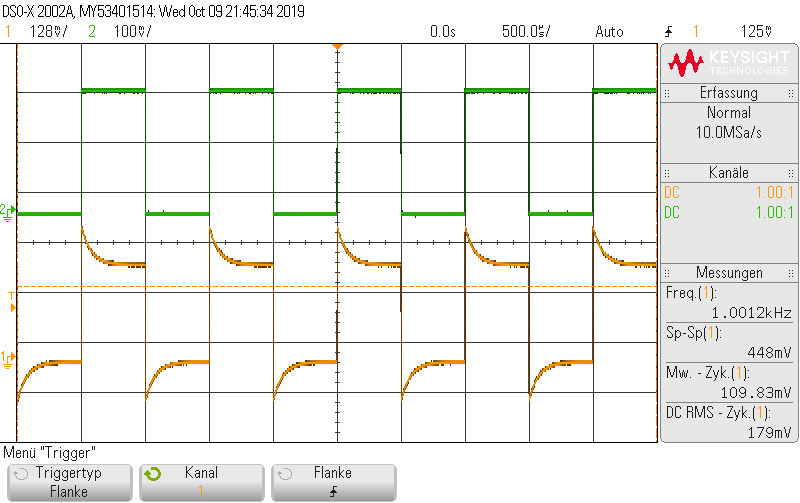
\includegraphics[width=8cm]{img/UeKomp}
			\subcaption{Überkompensiert}
		\end{subfigure}
		\caption{Spannungsverläufe}
	\end{figure}
	\newpage
	\noindent
	\underline{\textbf{Verhalten bei Sinusspannungen unterschiedlicher Frequenzen}} \\ \\
	Nun wird eine Sinusspannung mit steigender Frequenz (Dekaden-Schritte) gemessen. Diese Messung wird für einen über-, unterkompensierten und abgeglichenen Tastkopf durchgeführt. Gemessen wird die Spitze-Spitze-Spannung. Die Einstellung der Spannung am Frequenzgenerator war $10V_{pp}$.
	\begin{table}[h]
		\centering
		\begin{tabular}{|c|c|c|c|}
			\hline
			\multirow{2}{*}{$f[Hz]$} & \multirow{2}{*}{$U_{abgeglichen}[V]$} & \multirow{2}{*}{$U_{unterkomp}$} & \multirow{2}{*}{$U_{ueberkomp}$} \\
			&  &  &  \\ \hline
			\multirow{2}{*}{$100$} & \multirow{2}{*}{$10.125$} & \multirow{2}{*}{$10.56$} & \multirow{2}{*}{$10.4375$} \\
			&  &  &  \\ \hline
			\multirow{2}{*}{$1k$} & \multirow{2}{*}{$10.125$} & \multirow{2}{*}{$10.125$} & \multirow{2}{*}{$11.0625$} \\
			&  &  &  \\ \hline
			\multirow{2}{*}{$10k$} & \multirow{2}{*}{$10.125$} & \multirow{2}{*}{$7.175$} & \multirow{2}{*}{$13.4375$} \\
			&  &  &  \\ \hline
			\multirow{2}{*}{$100k$} & \multirow{2}{*}{$10.15$} & \multirow{2}{*}{$7.000$} & \multirow{2}{*}{$13.75$} \\
			&  &  &  \\ \hline
		\end{tabular}
		\caption{Auswertung von 2.2.1 Punkt 3}
	\end{table}
	\newline
	Aus Tabelle 8 ist ersichtlich, dass sich die Spannungswerte bei den nicht abgeglichen Tastköpfen mit steigender Frequenz von der Ursprungsspannung abweichen. Diese Spannungsänderung ergibt sich dadurch, das die verstellbare Kapazität des Tastkopfes nicht auf die Kapazität des Oszilloskopeinganges abgeglichen ist. Aus dem Messergebnis folgt das mit steigender Frequenz der Einfluss der Tastkopfkapazität zunimmt.
	\newpage
	\noindent
	\textbf{Weitere Erkenntnisse:} \\ \\
	Nun wird am Funktionsgenerator eine Sinusspannung mit einer Frequenz von $10kHz$ und einer Spannung von $10V_{pp}$ eingestellt. Anschließend werden die Spannungsverläufe von einen abgeglichenen und nicht abgeglichenen Tastkopf, in unserem Fall überkompensiert, mit dem Oszilloskop aufgenommen. 
	\begin{figure}[h]
		\centering
		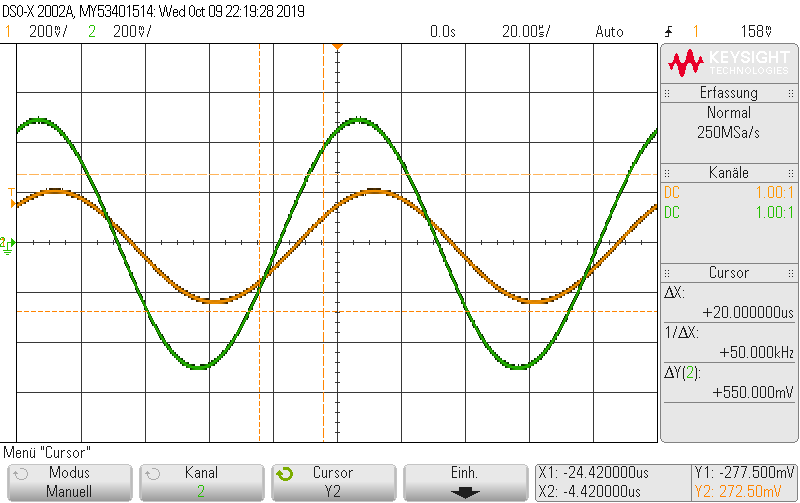
\includegraphics[width=10cm]{img/Phasenverschiebung}
		\caption{Vergleich Abgeglichen mit Überkompensiert}
	\end{figure}
	\newline
	Neben dem unterschiedlichen Wert der Spitze-Spitze-Spannung ist auch noch eine Phasenverschiebung zu erkennen. Diese beruht darauf, dass wir im nicht abgeglichenen Fall keine rein ohmsche sondern eine ohmsch-kapazitive Last.
	\newpage
	\subsubsection{AC-Spannungsmessung}
	\underline{\textbf{Aufgabenstellung}} \\ \\
	Die Aufgabe bei dieser Messung besteht darin, die Spannung am Widerstand $R_2$ (siehe Abb.11), bei verschieden Signalformen und unterschiedlichen Frequenzen zu messen. Der Spitze-Spitze-Wert zu soll gemessen und daraus der Effektivwert berechnet werden. Außerdem sollen die Messungen einmal für die Einstellung High-Z und $50\Omega$ am Oszilloskop durchgeführt werden.
	\begin{figure}[h]
		\centering
		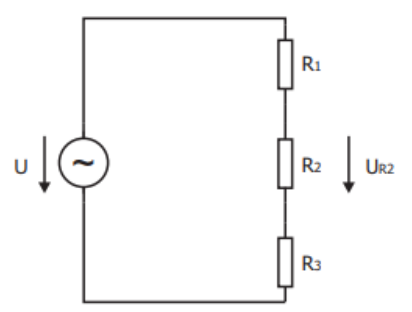
\includegraphics[width=8cm]{img/AC-Spannungsmessung}
		\caption{Schaltung zur AC-Spannungsmessung an $R_2$}
	\end{figure}
	\newline
	\underline{\textbf{Messdurchführung}} \\ \\
	Die Schaltung soll mit $R_1 = 100\Omega$, $R_2 = 4.7k\Omega$ und $R_3 = 100k\Omega$ aufgebaut. Bevor sie aufgebaut wurde, sind die genauen Widerstandswerte mit dem Ohmmeter bestimmt worden. Diese betrugen $99.6\Omega$, $4.709k\Omega$ und $102.9k\Omega$. Der Spannungswert am Funktionsgenerator betrug bei jeder Messung $10V_{pp}$. \\
	\noindent
	Prinzipiell gibt es verschiedene Arten die Spannung an $R_2$ zu messen. Die erste besteht darin die Spannungen an $R_2$ und $R_3$ und $R_3$ selbst zu messen. Dies muss so durchgeführt, da das hier verwendete Oszilloskop nur Spannung gegen Masse aufnehmen kann. Anschließend wird mittels der \textit{Math}-Funktion des Oszilloskop die Differenz der beiden Spannung berechnet und man erhält die gesuchte Spannung. \\
	\noindent
	Die zweite Messart besteht darin, die Widerstände $R_2$ und $R_3$ einfach zu vertauschen und dann einfach direkt die Spannung am Widerstand $R_2$ messen und mit dem Oszilloskop aufnehmen.
	\newpage
	\noindent
	Der Effektivwert der Signale  wird wie folgt bestimmt:
	\[
		U_{RMS} = \frac{\frac{U_{pp}}{2}}{k_s}
	\]
	Der Wert $k_s$ heißt \textit{Crest-Faktor} und lautet für unsere zu verwendenden Signale:
	\begin{align*}
		k&_{s,sin} = \sqrt{2} \\
		k&_{s,Dreieck} = \sqrt{3} \\
		k&_{s,Rechteck} = 1
	\end{align*}
	\begin{table}[h]
		\centering
		\begin{tabular}{|c|c|c|c|c|c|}
			\hline
			\multirow{2}{*}{$f[kHz]$} & \multirow{2}{*}{Signalform} & \multirow{2}{*}{$U_{pp,HighZ}[V]$} & \multirow{2}{*}{$U_{pp,50\Omega}[V]$} & \multirow{2}{*}{$U_{RMS,HighZ}[V]$} & \multirow{2}{*}{$U_{RMS,50\Omega}[V]$} \\
			&  &  &  &  &  \\ \hline
			\multirow{2}{*}{$1$} & \multirow{2}{*}{Sinus} & \multirow{2}{*}{$0.470$} & \multirow{2}{*}{$0.900$} & \multirow{2}{*}{$0.156$} & \multirow{2}{*}{$0.312$} \\
			&  &  &  &  &  \\ \hline
			\multirow{2}{*}{$1$} & \multirow{2}{*}{Dreieck} & \multirow{2}{*}{$0.4525$} & \multirow{2}{*}{$0.890$} & \multirow{2}{*}{$0.128$} & \multirow{2}{*}{$0.254$} \\
			&  &  &  &  &  \\ \hline
			\multirow{2}{*}{$10$} & \multirow{2}{*}{Dreieck} & \multirow{2}{*}{$0.4525$} & \multirow{2}{*}{$0.890$} & \multirow{2}{*}{$0.128$} & \multirow{2}{*}{$0.254$} \\
			&  &  &  &  &  \\ \hline
			\multirow{2}{*}{$100k$} & \multirow{2}{*}{Dreieck} & \multirow{2}{*}{$0.465$} & \multirow{2}{*}{$0.900$} & \multirow{2}{*}{$0.129$} & \multirow{2}{*}{$0.256$} \\
			&  &  &  &  &  \\ \hline
			\multirow{2}{*}{$1$} & \multirow{2}{*}{Rechteck} & \multirow{2}{*}{$0.4625$} & \multirow{2}{*}{$0.9315$} & \multirow{2}{*}{$0.220$} & \multirow{2}{*}{$0.443$} \\
			&  &  &  &  &  \\ \hline
			\multirow{2}{*}{$10$} & \multirow{2}{*}{Rechteck} & \multirow{2}{*}{$0.4625$} & \multirow{2}{*}{$0.890$} & \multirow{2}{*}{$0.221$} & \multirow{2}{*}{$0.443$} \\
			&  &  &  &  &  \\ \hline
			\multirow{2}{*}{$100$} & \multirow{2}{*}{Rechteck} & \multirow{2}{*}{$0.4625$} & \multirow{2}{*}{$0.890$} & \multirow{2}{*}{$0.227$} & \multirow{2}{*}{$0.447$} \\
			&  &  &  &  &  \\ \hline
		\end{tabular}
	\caption{Auswertung von 2.2.2}
	\end{table}
	\newline
	Wir erwarten das der Spitze-Spitze- und der Effektivwert ca. doppelt so groß ist, wie bei der Einstellung \textit{HighZ}. Das kann man in der Tabelle 9 sehr gut erkennen. Die doppelte Spannung beruht darauf, das wir im Funktionsgenerator einstellen, dass wir unsere Leitung mit $50\Omega$ abgeschlossen haben. Dadurch das ein Spannungsteiler mit dem Innenwiderstand des Funktionsgenerator zustande kommt, fällt am Ausgang nurmehr die halbe Eingangsspannung ab. Deswegen stellt der Funktionsgenerator komplett automatisch die doppelte Spannung ein, welche wir dann auch messen.
	\newpage
	\subsubsection{RMS im Detail}
	\underline{\textbf{Aufgabenstellung}}\\ \\
	Hier soll von unterschiedlichen Signalformen bei verschiedenen Frequenzen der Effektivwert mit dem Oszilloskop und zwei verschiedenen Multimetern gemessen werden. Die zu messende Spannung soll eine Amplitude von $10V$ besitzen. \\ \\
	\underline{\textbf{Durchführung}}
	\begin{table}[h]
		\centering
		\begin{tabular}{|c|c|c|c|c|c|}
			\hline
			\multirow{2}{*}{$f[kHz]$} & \multirow{2}{*}{Signalform} & \multirow{2}{*}{$U_{pp,Oszi}[V]$} & \multirow{2}{*}{$U_{RMS,Oszi}[V]$} & \multirow{2}{*}{$U_{RMS,MM1}[V]$} & \multirow{2}{*}{$U_{RMS,MM2}[V]$} \\
			&  &  &  &  &  \\ \hline
			\multirow{2}{*}{$1$} & \multirow{2}{*}{Sinus} & \multirow{2}{*}{$20.1$} & \multirow{2}{*}{$7.06$} & \multirow{2}{*}{$7.04$} & \multirow{2}{*}{$7.02$} \\
			&  &  &  &  &  \\ \hline
			\multirow{2}{*}{$100$} & \multirow{2}{*}{Sinus} & \multirow{2}{*}{$20.1$} & \multirow{2}{*}{$7.04$} & \multirow{2}{*}{$6.98$} & \multirow{2}{*}{$0.125$} \\
			&  &  &  &  &  \\ \hline
			\multirow{2}{*}{$1000$} & \multirow{2}{*}{Sinus} & \multirow{2}{*}{$20$} & \multirow{2}{*}{$7$} & \multirow{2}{*}{$0.0029$} & \multirow{2}{*}{$0.0051$} \\
			&  &  &  &  &  \\ \hline
			\multirow{2}{*}{$1$} & \multirow{2}{*}{Rechteck} & \multirow{2}{*}{$20.3$} & \multirow{2}{*}{$9.97$} & \multirow{2}{*}{$9.85$} & \multirow{2}{*}{$9.85$} \\
			&  &  &  &  &  \\ \hline
			\multirow{2}{*}{$100$} & \multirow{2}{*}{Rechteck} & \multirow{2}{*}{$20.1$} & \multirow{2}{*}{$9.90$} & \multirow{2}{*}{$9.88$} & \multirow{2}{*}{$0.3731$} \\
			&  &  &  &  &  \\ \hline
			\multirow{2}{*}{$1000$} & \multirow{2}{*}{Rechteck} & \multirow{2}{*}{$20.1$} & \multirow{2}{*}{$9.6$} & \multirow{2}{*}{$0.001$} & \multirow{2}{*}{$0.001$} \\
			&  &  &  &  &  \\ \hline
			\multirow{2}{*}{$1$} & \multirow{2}{*}{Dreieck} & \multirow{2}{*}{$20.1$} & \multirow{2}{*}{$5.776$} & \multirow{2}{*}{$5.74$} & \multirow{2}{*}{$5.73$} \\
			&  &  &  &  &  \\ \hline
			\multirow{2}{*}{$100$} & \multirow{2}{*}{Dreieck} & \multirow{2}{*}{$20.1$} & \multirow{2}{*}{$5.75$} & \multirow{2}{*}{$5.67$} & \multirow{2}{*}{$0.060$} \\
			&  &  &  &  &  \\ \hline
			\multirow{2}{*}{$1000$} & \multirow{2}{*}{Dreieck} & \multirow{2}{*}{$19.9$} & \multirow{2}{*}{$5.75$} & \multirow{2}{*}{$1.494$} & \multirow{2}{*}{$1.894$} \\
			&  &  &  &  &  \\ \hline
		\end{tabular}
		\caption{Auswertung von 2.2.3}
	\end{table}
	\newline
	Für \textit{MM1} wurde das \textit{Agilent U1232A} und für \textit{MM2} wurde das \textit{Neumann 9140} verwendet. \\
	Annahme:
	\begin{align*}
		U&_{RMS} = \frac{\frac{U_{pp}}{2}}{k_s} \\
		k&_{s,sin} = \sqrt{2} \\
		k&_{s,Dreieck} = \sqrt{3} \\
		k&_{s,Rechteck} = 1
	\end{align*}
	\newline
	Die Messung hat unsere Erwartung großteils bestätigt. Es wurde festgestellt das beide Multimeter den Effektivwert verschiedener Signalformen bei der Frequenz von $1MHz$ nicht korrekt messen kann. Des Weiteren scheint \textit{MM2} nur bei $1kHz$ brauchbare Werte zu liefern. Außerdem kann es nicht den \textit{True-RMS} messen, da es ein Sinussignal voraussetzt und kann diesen auch nur in einem niedrigen Frequenzbereich messen.
	\subsubsection{Amplitudenauflösung}
	\underline{\textbf{Aufgabenstellung}} \\ \\
	In Teil soll die Auflösung (horizontal) des Oszilloskop bestimmt werden.\\ \\
	\underline{\textbf{Durchführung}} \\ \\
	Um die horizontale Auflsung festzustellen, wird ein Bild angehalten und zoomt in das Bild solange hinein bis man die einzelnen Steps (siehe Abb.12) sehen kann.
	\begin{figure}[h]
		\centering
		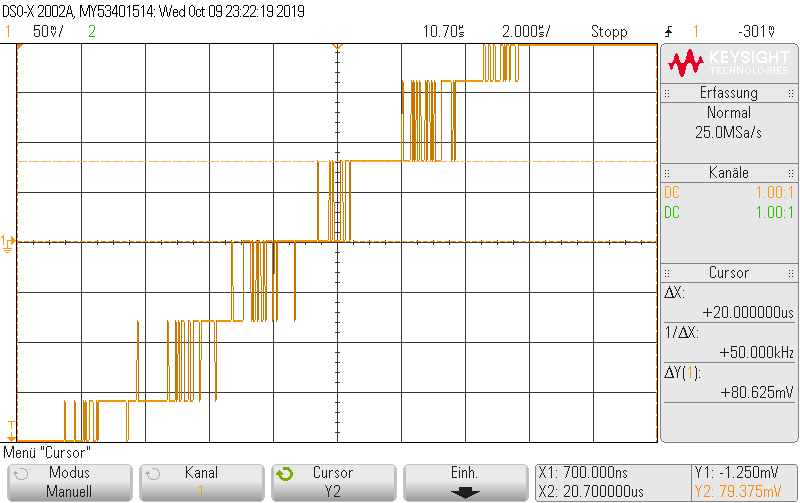
\includegraphics[width=10cm]{img/Auflo}
		\caption{Steps eines Sinus mit $5V$ bei $1kHz$}
	\end{figure}
	\newline
	Ist die Höhe des einzelnen Step und die maximale Höhe des Signals bekannt, kann aus diesen beiden Werten berechnet werden, wieviele Steps benötigt werden. Es wurde festgestellt das ein Bild 255 Steps hat, worauf man auf einen 8-Bit ADC schließen kann.
	\newpage
	\subsubsection{Dynamik}
	\underline{\textbf{Aufgabenstellung}} \\ \\
	Hier sollen die beiden unterschiedlichen Eingangskopplungen des Oszilloskopes untersucht werden. Diese sind die AC- und DC-Kopplung. \\ \\
	\underline{\textbf{Durchführung}} \\ \\
	Es wird ein Sinussignal mit $8Hz$ an zwei Eingänge des Oszilloskop angeschlossen. Channel 1 ist DC und Channel 2 ist AC gekoppelt.
	\begin{figure}[h]
		\centering
		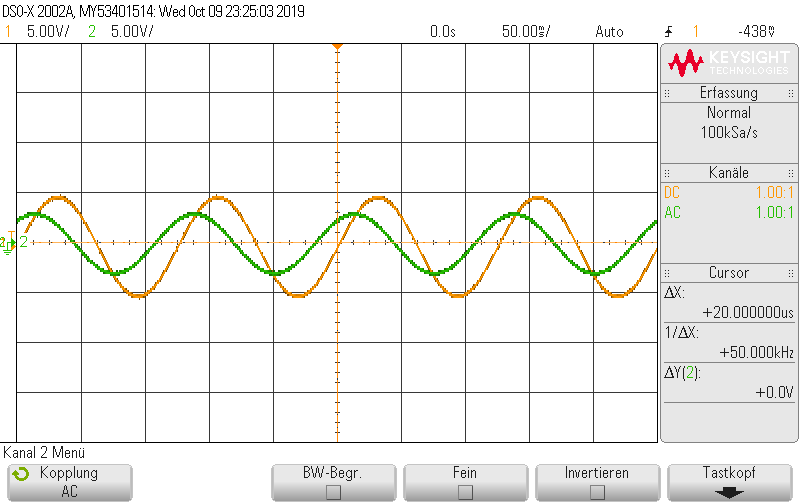
\includegraphics[width=12cm]{img/ACDC}
		\caption{Spannungsverläufe beider Kopplungsarten}
	\end{figure}
	\newline
	Man kann sehr gut erkennen, dass bei der AC-Kopplung die Spannung gedämpft wird. Das liegt daran, dass bei der AC-Kopplung ein Tiefpass dazwischen geschaltet wird, um Gleichanteile aus dem Signal herauszufiltern.
	\newpage
	\subsubsection{Einschaltvorgang Spannungsversorgung}
	\underline{\textbf{Aufgabenstellung}} \\ \\
	Hier soll der Einschaltvorgang der verwendeten Spannungsversorgung aufgenommen werden. \\ \\
	\underline{\textbf{Durchführung}}
	\begin{figure}[h]
		\centering
		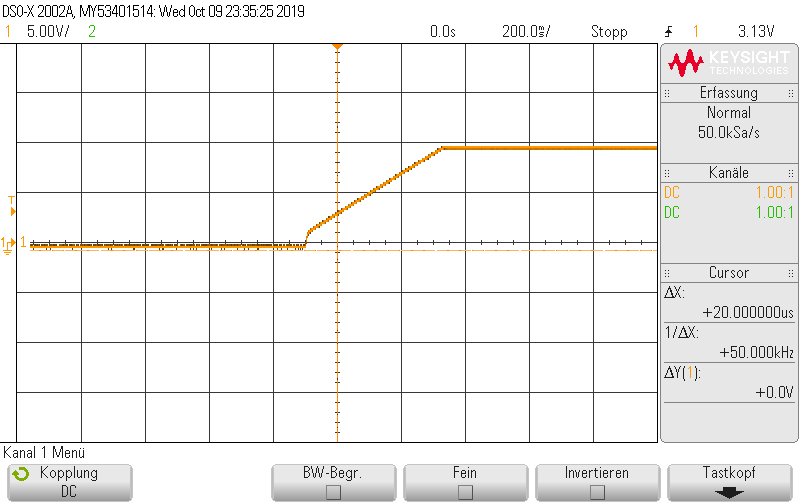
\includegraphics[width=12cm]{img/Einschaltvorgang}
		\caption{Einschaltvorgang mit Strombegrenzung}
	\end{figure}
    \newline
    Hier ist gut zu erkennen, das sich die Strombegrenzung der Spannungsquelle sich aktiviert hat, weil anfangs die Kurve exponentiell ansteigt und diese kurz darauf gebremst wird durch diese.
    \newpage
	\subsection{Messwerke}
	\underline{\textbf{Drehspulenmesswerk}} \\ \\
	Das Drehspulenmesswerk (siehe Abb.15) besitzt eine frei bewegliche Spule, welche mit dem zugeführten elektrischen Strom ein elektrisches Moment ausübt, was die Spule rotieren lässt. Um dieser Rotation (permanent) entgegenzuwirken, besitzt das Messwerk eine mechanische Feder, welche ein mechanisches Moment entsprechend dem Auslenkungswinkel ausübt. Sind das elektrische und mechanische Moment im Gleichgewicht, kommt die Spule zum Stillstand und der Zeiger markiert den entsprechenden Strom auf der Skala.
	\begin{figure}[h]
		\centering
		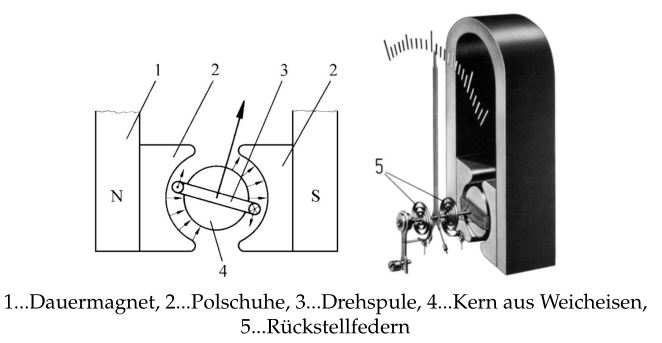
\includegraphics[width=15cm]{img/Drehspulenmesswerk}
		\caption{Aufbau eines Drehspulenmesswerkes}
	\end{figure}
	\newpage
	\noindent
	\underline{\textbf{Dreheisenmesswerk}} \\ \\
	Das Dreheisenmesswerk (siehe Abb.16) besitzt eine fest stehende Spule, welche die zwei sich im Inneren befindenden Eisenplättchen magnetisiert. Da beide Plättchen in gleicher Richtung magnetisiert werden, stoßen sich diese auch ab, wobei die dabei entstehende Kraft dem Produkt der einzelnen magnetischen Momente proportional ist. Da das magnetische Kraft von I abhängt, ist die resultierende Kraft von I$^2$, was bei einseitig schmäler werdenden Plättchen zu einem linearen Zusammenhang reduziert werden kann. Genauso wie beim Drehspulenmesswerk besitzt auch das Dreheisenmesswerk, welche der resultierenden Kraft entgegenwirkt um eine ruhende Position des Zeigers einzustellen.
	\begin{figure}[h]
		\centering
		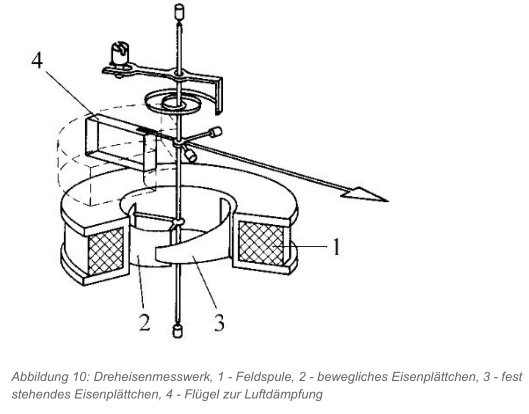
\includegraphics[width=15cm]{img/Dreheisen}
		\caption{Aufbau eines Dreheisenmesswerkes}
	\end{figure}
	
	\newpage
	\section{Verwendete Geräte}
	\begin{itemize}
		\item DP862 Programmable DC Power Supply
		\item Agilent U1232A (True RMS Multimeter)
		\item DSO-X-2002A (Digital Storage Oscilloscope)
		\item SDG1025 (Function/Arbittaey Waveform Generator)
		\item NEUMANN 9140 (Multimeter)
	\end{itemize}
	\newpage
	\listoffigures
	\newpage
	\listoftables
\end{document}